% !TEX TS-program = xelatex
\documentclass[11pt]{article}
%\pdfcompresslevel=0
%\pdfgentounicode=1 
%\input glyphtounicode.tex 
%\InputIfFileExists{glyphtounicode-cmr.tex}{}{} 
%\InputIfFileExists{glyphtounicode-ntx.tex}{}{}
%\usepackage[a-1b]{pdfx} % version 1.6.4 or higher
\usepackage{trace}
\usepackage[margin=1in]{geometry} 
\usepackage[parfill]{parskip} 
\usepackage{graphicx,xcolor}
\ifluatex\else%
\ifxetex\pdfmapfile{+XCharter.map}\pdfmapfile{+newtx.map}%
\else
\pdfmapfile{=XCharter.map}\pdfmapfile{=newtx.map}%
\fi\fi
\usepackage[scaled=1.03,varqu,varl]{inconsolata}
\usepackage[type1]{cabin}
\usepackage[OT2,T2A,T1]{fontenc}
%\traceon
\usepackage[xcharter,osf,p,mathscale=1.05,textscale=0,uprightscript,vvarbb]{newtx}
%\usepackage[scaled=.98,osf,otfmath]{XCharter}
\iftutex\setmonofont{lmmono10-regular.otf}[Scale=1.08]\fi
%\linespread{1.04}
%\usepackage[uprightscript,vvarbb,scaled=1.05]{newtxmath}
%\usepackage[cal=boondoxo]{mathalfa}
\makeatother
\iftutex
  \newfontface\osffnt{XCharter-Roman}[Numbers={Proportional,OldStyle}, CharacterVariant={1:0}]% , Scale = \XCharter@scale]
  \newfontface\osfIfnt{XCharter-Roman}[Numbers={Proportional,OldStyle}]%, Scale = \XCharter@scale]
\else
  \font\osfIfnt=XCharter-Roman-osf-t1 at 11pt
  \font\osffnt=XCharter1-Roman-osf-t1 at 11pt
\fi
\makeatletter
\usepackage{fonttable}
\usepackage{booktabs}
\usepackage{url}
\def\Sha{{\usefont{OT2}{XCharter-TLF}{m}{n}\char88 }}
\newcommand\cyrtext{\fontfamily{XCharter-TLF}\fontencoding{OT2}\selectfont} % declaration
\DeclareTextFontCommand{\textcyr}{\cyrtext}  %macro with argument
%\usepackage[cal=rsfso]{mathalfa}
%\usepackage{bm}% load after all math to give access to bold math
\title{The XCharter Font Package}
\author{Michael Sharpe}
%\date{}
\begin{document}
%%\traceon
%{\addfontfeatures{RawFeature=+lnum;+tnum}0123456789}\\
%{\addfontfeatures{RawFeature=+lnum;+pnum}0123456789}\\
%{\addfontfeatures{RawFeature=+tnum}0123456789}\\
%0123456789\\
%{\addfontfeatures{Numbers={Lining,Tabular}}0123456789}\\
%{\addfontfeatures{Numbers={Lining,Proportional}}0123456789}\\
%{\addfontfeatures{Numbers={OldStyle,Monospaced}}0123456789}\\
%%\traceoff
%\end{document}
\maketitle
%\expandafter\show\csname oldstylenums \endcsname
%\traceon\oldstylenums{1}\traceoff
\section{Package Features}
The \emph{XCharter} fonts are extensions of the Bitstream Charter fonts, adding oldstyle figures, superior figures and small caps in all styles. The original Charter fonts were created by famed font designer Matthew Carter in the late 1980's to enhance legibility of the output from printers of that era (laser, dot matrix, thermal and inkjet) with resolutions that would now be considered low---not far from modern screen resolutions. Their low contrasts, high x-heights and use of piecewise linear outlines where possible may make them interesting again as fonts that will render well on small devices and perhaps projected slides. (It's worth noting that the same designer provided Georgia for Microsoft. It is widely considered to be one of the clearest serifed fonts for viewing on screen, and bears a number of similarities to Charter, though the latter is  heavier.) 

As of version 1.09 (2017-06-25) there is a new collection of Cyrillic glyphs in \emph{XCharter}, copied from Andrey Panov's \emph{Khartiya}, an extension of the free Charter fonts, with small caps included. Some new figure styles were also copied from \emph{Khartiya}---inferiors, numerators and denominators. Along with these additions, there are now slanted versions for those who wish to have both slanted and italic text available to meet distinct semantic purposes. Note that figures and uppercase slanted and italic are almost identical (except for slanted \textsl{Q} and italic \textit{Q}) but lower-case forms are distinct.

Starting with version 1.1, support has been added for typesetting in the Serbian variant of Cyrillic, with some changes to the Italic and BoldItalic Cyrillic glyphs and a new option in the main package. These are described more fully below.

Support files are provided for T$1$, TS$1$, LY$1$, T$2$A and OT$2$ encodings, the last two being to support the Cyrillic component of \emph{XCharter}. The package has  a number of options:
\begin{itemize}
\item
{\tt scaled=.98}, for example, scales all text to 98\% of specified size;
\item {\tt lining} (or just {\tt lf}) makes lining figures ($0123456789$) the default for text---this is set automatically and does not need to be entered explicitly;
\item {\tt oldstyle} (or {\tt osf}) sets the figure style in text mode to oldstyle ({\osffnt  0123456789}) with numeral one like a shortened  $1$, but math mode will always use lining figures;
\item {\tt proportional} (or {\tt p}), new as of version 1.23, changes the default tabular figure style to proportional.
\item {\tt oldstyleI} (or {\tt osfI}) sets the figure style in text mode to oldstyle ({\osfIfnt0123456789}) with numeral one like a shortened I, but math mode will always use lining figures;
\item {\tt sups} sets the style for superscript figures (e.g., footnote markers) to XCharter's superior figures rather than using the default text inserts in mathematical superscripts. This option has no effect if a KOMA class is in force.
\item {\tt scosf} makes oldstyle figures the default in small cap text, no matter what the global figure setting may be.
\item {\tt serbianc} is useful only with the T$2$A encoding. It modifies
one slot in upright and slanted shapes and five slots in italic shapes, as expected in Serbian Cyrillic. See the last section for examples.
\end{itemize}
\subsection*{Changes in version 1.23}
There are some substantial additions in version 1.23, some requiring {\tt newtx}, version 1.71 or higher:
\begin{itemize}
\item
{\tt XCharter.sty} now works with all flavors of LaTeX---unicode and non-unicode---but there may be some small differences in output. Essentially all previous  options and macros are supported and there are new ones available, some of which are limited to unicode engines.
\item Previous versions of {\tt XCharter} had only two normal figure styles: {\tt tabular lining} (the default) and {\tt proportional oldstyle}. Version 1.23 adds two more so there are separate {\tt TLF (tabular lining figures)}, {\tt LF (proportional lining figures)}, {\tt TOsF (tabular oldstyle figures)} and {\tt OsF (proportional oldstyle figures)}. Two new options have been added to globally select the default figures style. Option {\tt p} (or {\tt proportional}) and {\tt t} (or {\tt tabular}). A new command \verb|\useproportional| (preamble only) has the same effect as option {\tt proportional}.
\item With the new figures came new macros to select them, no matter what the defaults may be. There are two forms, one that switches the figures until further notice and the other a macro with an argument.
\begin{center}
  \begin{tabular}{@{} cccc @{}}
    \toprule
    Switch& Command & Effect & Example \\ 
    \midrule
    \verb|\tlfstyle| &\verb|\texttlf| & TLF & \verb|{\tlfstyle123}, \texttlf{123}| \\ 
    \verb|\lfstyle| &\verb|\textlf| & LF & \verb|{\lfstyle123},\textlf{123}| \\ 
   \verb|\tosfstyle| &\verb|\texttosf| & TOsF & \verb|{\tosfstyle123},\texttosf{123}| \\ 
  \verb|\osfstyle| &\verb|\textosf| & OsF & \verb|{\osfstyle123}, \textosf{123}| \\ 
    \bottomrule
  \end{tabular}
\end{center}
There are also the text font switches \verb|\liningnums|, \verb|\tabularnums|, \verb|\oldstylenums| and \verb|\proportionalnums|, each of which changes only one attribute of the figure style and alignment. For example, \verb|\liningnums| changes the style to {\tt lining} and \verb|\tabularnums| changes the figure alignment to {\tt tabular}.
\item
There is a theorem font option similar to those in newtx and newpx. A new font family, {\tt XCharterTH}, is made from the italic and bold italic faces of {\tt XCharter}, but having upright figures and punctuation that, IMO, look better than slanted ones in theorem statements and the like. For details, consult the brief descriptions below and the more discursive version in the documentation to {\tt newtx}. There is a {\tt theoremfont} option to {\tt XCharter} that works exactly the same as in {\tt newtx}.
\item The figure style in {\tt theoremfont} will by default be the same as your chosen figure style. Option {\tt thmlining} will ensure that lining figures are always used.
\item {\tt oldSS} specifies the preference for the old Capital Sharp S rather than the newer form, {\tt U+1E9E}\iftutex, \SS\fi.
\item There are new options that affect only unicode engines:
\begin{itemize}
\item
{\tt nofontspec} prevents {\tt XCharter.sty} from loading {\tt fontspec}.
\item {\tt type1text} (or {\tt type1})  specifies processing the text font using {\tt type1} mode. This does not prevent {\tt fontspec} from loading.
\item {\tt defaultfeatures=} gives you a place to set the default text font features for {\tt fontspec}.
\end{itemize}
\end{itemize}



\textsc{Special Macros:}
\begin{itemize}
\item \verb|\useproportional| (usable only in the preamble)  may be used for changing the text figure alignment to {\tt proportional} though math mode will use tabular lining figures. (New in 1.23.)
\item
\verb|\useosf| (usable only in the preamble) may be used for changing the text figure style to {\tt osf} though math mode will use lining figures.
\item \verb|\useosfI| (usable only in the preamble) may be used for changing the text figure style to {\tt osfI} though math mode will use lining figures.
\item \verb|\textsu| prints its argument in superior figures, e.g., \verb|\textsu{12}| results in \textsu{12}. The effect is the same with \verb|{\sustyle 12}|.
\item \verb|\textinf| prints its argument in inferior figures, e.g., \verb|\textinf{12}| results in \textinf{12}. The effect is the same with \verb|{\instyle 12}|. (In versions of {\tt XCharter} prior to $1.221$, \verb|\textinf| was named \verb|\textin|, but the latter conflicts with {\tt hyperref} which redefines it to point to U+2208.)
\item \verb|\textlf| prints its argument in lining figures, e.g., \verb|\textlf{12}| results in \textlf{12}. The effect is the same with \verb|{\lfstyle 12}|.
\item \verb|{\osfstyle 23}| prints \textosf{23} ({\tt OldStyle,Proportional}) while \verb|{\liningnums 23}| prints {\liningnums 23}, {\tt Lining} with whatever figure alignment is in force. There are also macros \verb|\tabularnums|, \verb|\proportionalnums|, \verb|\oldstylenums|, \verb|\tosfstyle| and \verb|\tlfstyle| with the expected behaviors.
%\item \verb|\textosf| prints its argument in oldstyle figures using, in effect, the {\tt osf} option---e.g., \verb|\textosf{12}| results in \textosf{12}. 
%\item \verb|\textosfI| prints its argument in oldstyle figures using, in effect, the {\tt osfI} option---e.g., \verb|\textosfI{12}| results in \textosfI{12}. 
\item Numerators and denominators are normally used only for constructing fractions, but may if needed be called using \verb|\textnumerator| and \verb|\textdenominator|. They are about 7\% smaller than superiors and inferiors. You may use \verb|\textde| and \verb|\textnu| as abbreviations, though the latter will not be available if {\tt babel} is loaded with {\tt greek} option. As of version 1.24, you may prevent \verb|\textnu| from overwriting the babel/greek definition by using the new option {\tt notextnu} to {\tt XCharter}. In any case, a new command \verb|\textnum| takes the place of the old {\tt XCharter} \verb|\textnu|.
\item The \verb|\textfrac| macro allows you to write, e.g.,  \verb|\textfrac{31}{32}| to get the simple fraction \textfrac{31}{32}, and \verb|\textfrac[2]{31}{32}| to get \textfrac[2]{31}{32}. (The optional argument, $2$ in the latter case, is always typeset in lining figures.)
\item The \verb|\textsfrac| macro, available only when you use the {\tt newtx} package with option {\tt xcharter} to load {\tt XCharter} with {\tt newtxmath}, allows you to write, e.g.,  \verb|\textsfrac{31}{32}| to get the simple stacked fraction 
\iftutex
\textsfrac{31}{32},\fi
 and \verb|\textsfrac[2]{31}{32}| 
 \iftutex
 to get \textsfrac[2]{31}{32}\fi%
 . (The optional argument, $2$ in the latter case, is always typeset in lining figures.)

\item \verb|\textcircled| renders its argument in raised and reduced small caps encircled by the {\tt bigcircle} glyph. E.g., \verb|\textcircled{M}| and \verb|\textcircled{m}| both render as \textcircled{M}. The macro works also for numerals: \verb|\textcircled{2}| renders as \textcircled{2}.
\item \verb|\textth| (and also \verb|\textthit|) render their arguments using the theorem fonts. For example:\\ 
\verb|\textth{Theorem font (01234):!}| renders as \textth{Theorem font (01234):!}---note the upright figures and punctuation. (There is no Bold theorem font---\verb|\textbf{\textth{Theorem font (01234):!}}| renders as \textbf{\textth{Theorem font (01234):!}}.) The related font switch \verb|\thfamily| is defined so that \verb|{\thfamily A12!}| and \verb|\textth{A12!}| are equivalent.  In opentype processing, the {\tt StylisticSet 05} controls whether  figures and punctuation are upright in italic shaped faces.

\end{itemize}
\subsection*{Math package choices:}

There is now a unicode math package, {\tt XCharter-Math} that may be run with a simple preamble containing
\begin{verbatim}
\usepackage{fontspec}
\setmainfont{XCharter} % reads XCharter.fontspec
\usepackage{unicode-math}
\setmathfont{XCharter-Math.otf}
\end{verbatim}
or, even better, as described in the documentation for {\tt XCharter-Math},
\begin{verbatim}
\usepackage{xcharter-otf}
\end{verbatim}
but in order to get the options and macros described in this documentation, you should use instead, for the same effect
\begin{verbatim}
\usepackage[otfmath]{XCharter} 
% loads fontspec, unicode-math, and sets XCharter-Math.otf
\end{verbatim}
\textsc{Notes on the last preamble fragment:}
\begin{itemize}
\item
Unless option {\tt otfmath} is specified,  math will be processed by {\tt newtxmath} with {\tt xcharter} option. (See examples 2--6 below.)
\item All options passed to {\tt XCharter} that are not understood by {\tt XCharter} will be passed along to {\tt xcharter-otf} provided option {\tt otfmath} was specified. 
\end{itemize}
Three non-unicode math packages seem to provide reasonable companions for \textsf{XCharter}. The first example uses Charter italics as math italics, but doesn't provide arbitrary scaling and doesn't sufficiently distinguish math italic v from mathematical Greek \verb|\nu|. Moreover, it is not easy to redefine \verb|\mathcal| to get a better math calligraphic alphabet---e.g., the {\tt mathalpha} package fails. The second uses \textsf{libertine} italics and Greek in math mode, which is a good match to Charter in style and weight after scaling up, is arbitrarily scalable, has distinct math italic v and mathematical Greek \verb|\nu|, and is completely compatible with {\tt mathalpha}. The third is a new revision of {\tt newtxmath} with option {\tt charter} (or, equivalently, {\tt xcharter}), which substitutes Charter italics as math italics and, as of version 1.11,  uses a newly developed family of Greek symbols in \{regular, bold\} $\times$ \{upright, italic\} to match the style and italic angle of XCharter. This version is scalable and has a math italic v (plus a matching w) distinct from \verb|\nu|. (The option {\tt noxchvw} to {\tt newtxmath} changes the v and w to be the original Charter italic glyphs, which may lead to issues with \verb|\nu|.)
% The option {\tt alty} to {\tt newtxmath/charter}, new as of version {\tt 1.203}, substitutes $y$ for the default \emph{y} which, IMO, works better in combination with other math symbols because it lacks the problematic tail of \emph{y}.)
%\newpage

\textsc{Example 1:}
\begin{verbatim}
% [pdf]latex only
\usepackage[charter,expert]{mathdesign}
\usepackage[scaled=.96,osf]{XCharter}% matches the size used in math
\linespread{1.04}
\end{verbatim}

\textsc{Example 2:}
\begin{verbatim}
% [pdf]latex only
\usepackage[scaled=.98,sups,osf]{XCharter}% lining figures in math, osf in text
\usepackage[scaled=1.04,varqu,varl]{inconsolata}% inconsolata typewriter
\usepackage[type1]{cabin}% sans serif
\usepackage[uprightscript,libertine,vvarbb,scaled=1.05]{newtxmath}
\linespread{1.04}
\end{verbatim}

\textsc{Example 3:}
\begin{verbatim}
% [pdf]latex only
\usepackage[scaled=.98,sups,osf]{XCharter}% lining figures in math, osf in text
\usepackage[scaled=1.04,varqu,varl]{inconsolata}% inconsolata typewriter
\usepackage[type1]{cabin}% sans serif
\usepackage[uprightscript,charter,vvarbb,scaled=1.05]{newtxmath}
\linespread{1.04}
\end{verbatim}
\textsc{Example 4:}
\begin{verbatim}
% [pdf]latex only
\usepackage[<specify babel languages>]{babel}% load before XCharter
\usepackage[scaled=.98,sups,osf]{XCharter}% osf in text, lining figures in math
\usepackage[scaled=1.04,varqu,varl]{inconsolata}% inconsolata typewriter
\usepackage[type1]{cabin}% sans serif
\usepackage[uprightscript,charter,vvarbb,scaled=1.05]{newtxmath}
\linespread{1.04}
\end{verbatim}

\textsc{Example 5:}
\begin{verbatim}
% an example using newtx.sty, works with all latex engines
\usepackage[<specify babel languages>]{babel}% load before newtx
\usepackage[scaled=1.04,varqu,varl]{inconsolata}% inconsolata tt
\usepackage[type1]{cabin}% sans serif for math
\usepackage[T1]{fontenc} % encoding to use for mathtt, etc
\usepackage[xcharter,osf,p,mathscale=1.05,textscale=0,uprightscript,vvarbb]{newtx}% loads newtxmath
% newtx loads fontspec with unicode engines
\setmonofont{lmmono10-regular.otf}[Scale=1.08] % typewriter for text
\linespread{1.04}
% load polyglossia after newtx, if using
\end{verbatim}

\textsc{Example 6:}
\begin{verbatim}
% Adds instructions to produce a pdf conforming to PDF/A-1b
%\pdfcompresslevel=0 % uncomment for debugging the pdf
%\pdfgentounicode=1 
%\input glyphtounicode.tex  % now part of latex
\InputIfFileExists{glyphtounicode-cmr.tex}{}{} 
\InputIfFileExists{glyphtounicode-ntx.tex}{}{}
\usepackage[a-1b]{pdfx} % version 1.6.4 or higher
\usepackage[<specify babel languages>]{babel}% load before XCharter
\usepackage[scaled=.98,sups,osf]{XCharter}% osf in text, lining figures in math
\usepackage[scaled=1.04,varqu,varl]{inconsolata}% inconsolata typewriter
\usepackage[type1]{cabin}% sans serif
\usepackage[uprightscript,charter,vvarbb,scaled=1.05]{newtxmath}
\linespread{1.04}
\end{verbatim}

Here is a short sample based on the preamble of \textsc{Example 3}:\\[4pt]
\def\Pr{\ensuremath{\mathbb{P}}}
\def\rmd{\mathrm{d}}
The typeset math below follows the ISO recommendations that only variables
be set in italic. Note the use of upright shapes for $\rmd$, $\mathrm{e}$
and $\uppi$. (The first two are entered as \verb|\mathrm{d}| and
\verb|\mathrm{e}|, and in fonts derived from {\tt newtxmath} or {\tt mtpro2},
 the latter is entered as \verb|\uppi|.)

\textbf{Simplest form of the \textit{Central Limit Theorem}:} \textit{Let
$X_1$, $X_2,\cdots$ be a sequence of iid random variables with mean $0$ 
and variance $1$ on a probability space $(\Omega,\mathcal{F},\Pr)$. Then}
\[\Pr\left(\frac{X_1+\cdots+X_n}{\sqrt{n}}\le y\right)\to\mathfrak{N}(y)\coloneq
\int_{-\infty}^y \frac{\mathrm{e}^{-v^2/2}}{\sqrt{2\uppi}}\,
\mathrm{d}v\quad\mbox{as $n\to\infty$,}\]
\textit{or, equivalently, letting} $S_n\coloneq\sum_1^n X_k$,
\[\mathbb{E} f\left(S_n/\sqrt{n}\right)\to \int_{-\infty}^\infty f(v)
\frac{\mathrm{e}^{-v^2/2}}{\sqrt{2\uppi}}\,\mathrm{d}v
\quad\mbox{as $n\to\infty$, for every $f\in\mathrm{b}
\mathcal{C}(\mathbb{R})$.}\]

\def\testupgreek{%
  \test\Gamma \test\Delta 
  \test\Theta \test\Lambda \test\Xi \test\Pi \test\Sigma
  \test\Upsilon \test\Phi \test\Psi \test\Omega }

\def\testupgreekit{%
  \test\Gammait \test\Deltait 
  \test\Thetait \test\Lambdait \test\Xiit \test\Piit \test\Sigmait
  \test\Upsilonit \test\Phiit \test\Psiit \test\Omegait }
\def\testlowgreeki{%
  \test\alpha \test\beta \test\gamma \test\delta \test\epsilon
  \test\zeta \test\eta \test\theta \test\iota \test\kappa \test\lambda
  \test\mu }
\def\testlowgreekii{%
  \test\nu \test\xi \test o \test\pi \test\rho \test\sigma \test\tau
  \test\upsilon \test\phi \test\chi \test\psi \test\omega }
\def\testlowgreekiii{%
  \test\varepsilon \test\vartheta \test\varpi \test\varrho
  \test\varsigma \test\varphi \test\varkappa \test\ell \test\wp}
\def\testlowgreekiu{%
  \test\upalpha \test\upbeta \test\upgamma \test\updelta \test\upepsilon
  \test\upzeta \test\upeta \test\uptheta \test\upiota \test\upkappa \test\uplambda
  \test\upmu }
\def\testlowgreekiiu{%
  \test\upnu \test\upxi \test o \test\uppi \test\uprho \test\upsigma \test\uptau
  \test\upupsilon \test\upphi \test\upchi \test\uppsi \test\upomega }
\def\testlowgreekiiiu{%
  \test\upvarepsilon \test\upvartheta \test\upvarpi \test\upvarrho
  \test\upvarsigma \test\upvarphi \test\upvarkappa}
\def\testlowgreek{%
  \testlowgreeki\testlowgreekii\testlowgreekiii}
\def\testlowgreeku{%
  \testlowgreekiu\testlowgreekiiu\testlowgreekiiiu}
\def\test#1{\; #1}

%\newpage
\textbf{Greek letters in version 1.11:} \[\testupgreek\]
\[\testupgreekit\]
\[\testlowgreek\]
\[\testlowgreeku\]
{\boldmath
\[\testupgreek\]
\[\testupgreekit\]
\[\testlowgreek\]
\[\testlowgreeku\]
}
\section{Text effects under \texttt{fontaxes}}
This package loads the {\tt fontaxes} package in order to access italic and slanted small caps. You should pay attention to the fact that {\tt fontaxes} modifies the behavior of some basic \LaTeX\ text macros such as \verb|\textsc| and \verb|\textup|. Under normal \LaTeX, some text effects are combined, so that, for example, \verb|\textbf{\textit{a}}| produces bold italic {\tt a}, while other effects are not, e.g., \verb|\textsc{\textup{a}}| has the same effect as \verb|\textup{a}|, producing the letter {\tt a} in upright, not small cap, style. With {\tt fontaxes}, \verb|\textsc{\textup{a}}| produces instead upright small cap {\tt a}. It offers a macro \verb|\textulc| that undoes small caps, so that, e.g., \verb|\textsc{\textulc{a}}| produces {\tt a} in non-small cap mode, with whatever other style choices were in force, such as bold or italics.

\section{Text Companion Issues}
As of version $1.206$, {\tt XCharter} has essentially full support for {\tt textcomp} and there should be no issues in using any of the macros like \verb|\textregistered| and \verb|\textinterrobang| (\textregistered, \textinterrobang.)

\textsc{XCharter-Roman-ts1}
\fonttable{XCharter-Roman-ts1}
%\newpage
\section{Usage with fontspec}
Because the package supplies a file named {\tt XCharter.fontspec} whose contents list the {\tt otf} files that correspond to each of Regular, Bold, Italic, BoldItalic, Slanted and BoldSlanted, you may load XCharter with just
\begin{verbatim}
\usepackage{fontspec}
\setmainfont{XCharter}
\end{verbatim}
With unicode-encoded text, you will, in particular,  have complete access to the Cyrillic glyphs.

\section{XCharter and PDF/A}
There are a number of PDF/A validators available, though their outputs can and do differ when applied to the same document. I've tried the following.
\begin{itemize}
\item
Adobe Acrobat Pro. Almost all XCharter documents validate PDF/A-1b.
\item 
\url{https://www.pdf-online.com/osa/validate.aspx} is a free online validator. Almost all XCharter documents validate PDF/A-1b.
\item 
The free {\tt veraPDF} validator is much stricter. Recent documents produced using XCharter since version 1.24 have validated correctly. 
\end{itemize}
\newpage

\section{Using Cyrillic with pdflatex}
The OT$2$ encoding, now considered as obsolete because it is 7-bit, is nonetheless useful to scholars who wish to write short segments using a Cyrillic script from a Western keyboard. There are two means of doing this, one using control sequences for the characters (e.g., \verb|\CYRA| for Cyrillic A) and the other using ligatures to access the characters. Tables setting out the substitutions available may be consulted at \url{http://herbert.the-little-red-haired-girl.org/dvi/pdf/cyrillic.pdf}.

Note that, while the OT$2$ encoded font is complete, there are many gaps in the T$2$A encoded version, so that only Modern Russian and Ukrainian are fully covered, along with a number of characters from Old Russian and other Slavic languages.

%\fonttable{XCharter-Roman-tfl-ot2.tfm}
%{\usefont{OT2}{XCharter-TLF}{m}{n} \char"41}
\textsc{XCharter-Roman-tlf-ot2.tfm}:\\
\vspace*{-12pt}
\fonttable{XCharter-Roman-tlf-ot2}

This encoding contains the upright {\tt Sha} glyph in slot 88. This may be used in mathematical formulas by defining
\verb|\def\Sha{{\usefont{OT2}{XCharter-TLF}{m}{n}\char88 }}|
so that one may write \verb|$\text{\Sha}(A/K)$| for the  Tate–Shafarevich group $\text{\Sha}(A/K)$.

\textsc{Example OT$2$ Preamble:}

\begin{verbatim}
\documentclass{article} 
\usepackage[OT2,T1]{fontenc} % loads ot2enc.def
\newcommand\cyrtext{%
\fontfamily{XCharter-TLF}\fontencoding{OT2}\selectfont} % declaration
\DeclareTextFontCommand{\textcyr}{\cyrtext}  %macro with argument
\end{verbatim}
The Russian part of the following sentence is entered as \verb|\textcyr{a e1to --- po-russki}|.

This is text in English, then Russian:
\textcyr{a e1to --- po-russki}.
\newpage

\textsc{Using T$2$A with T$1$:}

Here's an example of using {\tt XCharter} text and math, set up to allow the use of  Russian with English as the main language.
\begin{verbatim}
\usepackage[OT2,T2A,T1]{fontenc} % spell out all text encodings to be used
\usepackage[utf8]{inputenc} % 
\usepackage{substitutefont} % so we can use fonts other than those specified in babel
\usepackage[russian,english]{babel}
\usepackage{XCharter} % 
\usepackage[charter,vvarbb,scaled=1.07]{newtxmath}
\useosf % use oldstyle figures except in math
\substitutefont{T2A}{\rmdefault}{XCharter} % use XCharter to render Russian 
%\substitutefont{OT2}{\rmdefault}{XCharter} % poor man's version
\end{verbatim}
Any {\tt utf8}-encoded text typed outside of a \verb|\foreignlanguage{}{}| block will be rendered as T$1$-encoded {\tt XCharter}, while that within \verb|\foreignlanguage{russian}{}| will render as T$2$A-encoded Cyrillic. 

\newpage
\textsc{XCharter-Roman-tlf-t2a.tfm}:\\
\fonttable{XCharter-Roman-tlf-t2a.tfm}
\newpage
\textsc{XCharter-Italic-tlf-t2a.tfm}:\\
\fonttable{XCharter-Italic-tlf-t2a.tfm}

\textsc{Note:} Currently, the \LaTeX\ support files for T$2$A encoded \emph{XCharter} cover only the figure styles {\tt lining}, {\tt oldstyle} and {\tt superiors}.
\section{Serbian Cyrillic}
Serbian and Russian Cyrillic differ in the following ways.

\font\russc=XCharter-Roman-tlf-t2a at 11pt
\font\serbc=XCharter-Roman-tlf-t2asrb at 11pt
\font\russci=XCharter-Italic-tlf-t2a at 11pt
\font\serbci=XCharter-Italic-tlf-t2asrb at 11pt
\begin{center} 
  \begin{tabular}{@{} cccc @{}}
    \toprule
    Character & Shape & Russian & Serbian \\ 
    \midrule
    U+0431 & Upright & {\russc\char"E1} & {\serbc\char"E1} \\ 
    U+0431 & Italic & {\russci\char"E1} & {\serbci\char"E1} \\ 
    U+0433 & Italic & {\russci\char"E3} & {\serbci\char"E3} \\ 
    U+0434 & Italic & {\russci\char"E4} & {\serbci\char"E4} \\ 
    U+043F & Italic & {\russci\char"EF} & {\serbci\char"EF} \\ 
    U+0442 & Italic & {\russci\char"F2} & {\serbci\char"F2} \\ 
   \bottomrule
  \end{tabular}
\end{center}

Usage under XeLaTeX and XeLaTeX is simple. Your preamble should include
\begin{verbatim}
\usepackage{polyglossia}
\usepackage{fontspec}
\setmainfont{XCharter}[%
Language=Serbian,
Script=Cyrillic
]
\end{verbatim}
Then all (unicode) input characters will be typeset using the above substitution table. 

The story is a bit more complicated with \LaTeX\ processing.
 
\textsc{Example 1: Serbian Cyrillic as default text.}
\begin{verbatim}
\usepackage[utf8x]{inputenc}
\usepackage[serbianc]{babel}
\usepackage[serbianc]{XCharter}
\usepackage[T2A]{fontenc}
\end{verbatim}
This will produce essentially the same output as the {\tt fontspec} example above, with unicode input.

It may be be possible to work out a scheme that would allow multiple scripts and languages to be used with {\tt serbianc} as the main or as a secondary language in {\tt babel}, but I have not succeeded in doing this with XCharter, and know of no other example that I might crib from.
%\textsc{Example 2: 

\section*{Opentype processing and German orthography}
Prior to version {\tt1.12}, {\tt XCharter} offered only basic support for German orthography, having all required accented glyphs and the lower case \ss, as well as a small caps \textsc{\ss}. Under non-unicode LaTeX, the T$1$ encoding contained \verb|S_S|. With unicode tex processing:
\begin{verbatim}
{\addfontfeature{StylisticSet=1}\ss\ \textsc{\ss}}
\end{verbatim}
typesets, as in non-unicode LaTeX processing, to

\ss\ \textsc{\ss}

Note also that in unicode processing, in order to obtain the expected case change behavior, it may be necessary to add in your preamble:
\begin{verbatim}
\uccode`ß="1E9E
\end{verbatim}


 As of version {\tt1.12} of {\tt XCharter}, there are now glyphs in each style for {\tt U+1E9E} and for its small caps version,  accessible under unicode TeX. The glyphs may be used as the uppercase and small caps versions of {\tt germandbls}. Currently, the new glyphs are not available in any of the LaTeX encodings and must be used via unicode TeX.

The following tables show how to access the new glyphs in unicode TeX. Note that you will need to set {\tt StylisticSet=1} if you wish not to use the new sharp-s glyphs.

%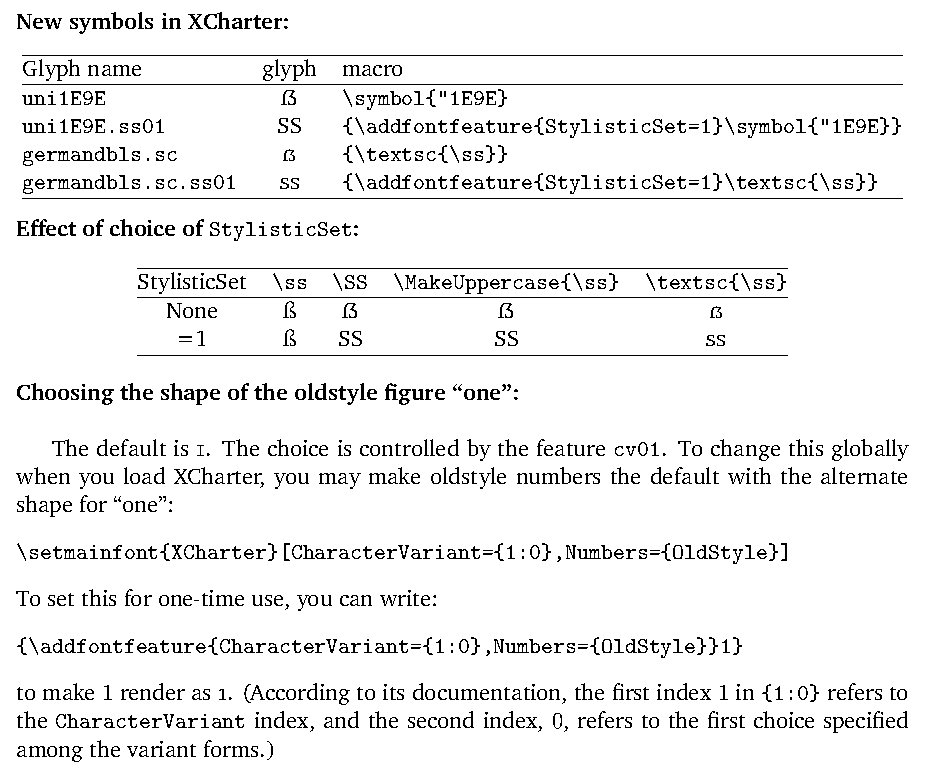
\includegraphics{newgermanfxch-crop}
\noindent \textbf{New symbols in XCharter:}
\begin{center}
  \begin{tabular}{@{} lcl @{}}
    \hline
    Glyph name & glyph & macro\\ 
    \hline
    {\tt uni1E9E} & \symbol{"1E9E} &\verb|\symbol{"1E9E}|\\ 
    {\tt uni1E9E.ss01} & {\addfontfeature{StylisticSet=1}\symbol{"1E9E}} & \verb|{\addfontfeature{StylisticSet=1}\symbol{"1E9E}}| \\ 
    {\tt germandbls.sc} & \textsc{\ss} & \verb|{\textsc{\ss}}| \\ 
    {\tt germandbls.sc.ss01} & {\addfontfeature{StylisticSet=1}\textsc{\ss}} & \verb|{\addfontfeature{StylisticSet=1}\textsc{\ss}}| \\ 
    \hline
  \end{tabular}
\end{center}  
 
%{\bfseries
%\begin{center}
%  \begin{tabular}{@{} lcl @{}}
%    \hline
%    Glyph name & glyph & macro\\ 
%    \hline
%    {\tt uni1E9E} & \symbol{"1E9E} &\verb|\symbol{"1E9E}|\\ 
%    {\tt uni1E9E.alt} & {\addfontfeature{StylisticSet=1}\symbol{"1E9E}} & \verb|{\addfontfeature{StylisticSet=1}\symbol{"1E9E}}| \\ 
%    {\tt germandbls.sc.ss02} & {\addfontfeature{StylisticSet=1}\textsc{\ss}} & \verb|{\addfontfeature{StylisticSet=1}\textsc{\ss}}| \\ 
%    \hline
%  \end{tabular}
%\end{center}
%}
\noindent \textbf{Effect of choice of {\tt StylisticSet}:}
 
\begin{center}
  \begin{tabular}{@{} ccccc @{}}
    \hline
    StylisticSet & \verb|\ss| & \verb|\SS| & \verb|\MakeUppercase{\ss}| & \verb|\textsc{\ss}| \\ 
    \hline
    None & \ss & \SS & \MakeUppercase{\ss} & \textsc{\ss}\\ 
    
    =1 & {\addfontfeature{StylisticSet=1}\ss} & {\addfontfeature{StylisticSet=1}\SS} & {\addfontfeature{StylisticSet=1}\MakeUppercase{\ss}} & {\addfontfeature{StylisticSet=1}\textsc{\ss}}\\ 
    \hline
  \end{tabular}
\end{center}

\noindent \textbf{Choosing the shape of the oldstyle figure ``one'':}\\

The default is \oldstylenums{1}. The choice is controlled by the feature \texttt{cv01}. To change this globally when you load XCharter, you may make oldstyle numbers the default with the alternate shape for ``one'':
\begin{verbatim}
\setmainfont{XCharter}[CharacterVariant={1:0},Numbers={OldStyle}]
\end{verbatim}
To set this for one-time use, you can write:
\begin{verbatim}
{\addfontfeature{CharacterVariant={1:0},Numbers={OldStyle}}1}
\end{verbatim}
to make $1$ render as {\addfontfeature{CharacterVariant={1:0},Numbers={OldStyle}}\oldstylenums{1}}. (According to its documentation, the first index $1$ in \verb|{1:0}| refers to the {\tt CharacterVariant} index, and the second index, $0$, refers to the first choice specified among the variant forms.)
%1{\addfontfeature{CharacterVariant={1:0},Numbers={OldStyle}}1}
%{\addfontfeature{CharacterVariant={1:1},Numbers={OldStyle}}1}

If you choose to load {\tt XCharter-*.otf} using {\tt XCharter.sty} or {\tt newtx}, you may make use of the options {\tt osf}, {\tt osfI} or the macros \verb|\useosf|, \verb|\useosfI| to the same effect.

\end{document}